\chapter{Prototype: Design}
The role of the user will be to play as a child with autism and experience the world through their eyes, obtaining valuable insight and understanding as to what it may feel like to have these difficulties reducing inference and guess-work from literature(probably better explained what I mean in the sound part of "Redesign").

The primary target audience selected are teachers however, it should be developed such that anyone with little knowledge on autism and computer game experience can play and learn. To further achieve this, accessibility is an important consideration and where possible it should be made freely available on-line, making autism training a fun and interactive possibility for all, regardless of budget.  

Finally, instead of creating an overall architecture for the prototype it was chosen to simply implement features and allow the system to evolve due to current limited experience with JMonkey; the architecture would be likely rapidly change as issues arise, voiding any plans or design. For the second iteration of the design; a more in-depth plan detailing components of the system should be created.

\section{Game play}

The user will move around and explores a realistic home environment and be able to interact with objects such as turning off lights, opening and closing doors. Their well-being will be monitored at all times by a $contentment$ gauge visible on screen. Certain actions will result in this reducing, i.e a sensory overload or getting dressed and other interactions such as engaging with a special interest will increase contentment. If contentment drops to zero the player experiences a meltdown and restarts. 

\subsection{Interface and Controls}

Contentment as in the top right of \ref{design_interface_actions} is represented as a "health bar". When the user aligns the cross hair with an object and presses the action button, an interface will pop up with the actions currently available. On the top left of \ref{design_interface_actions} is the tool tip which will change depending on what object the cross hair is hovered over, indicate if there are any actions available. 

\begin{figure}[H]
\centering
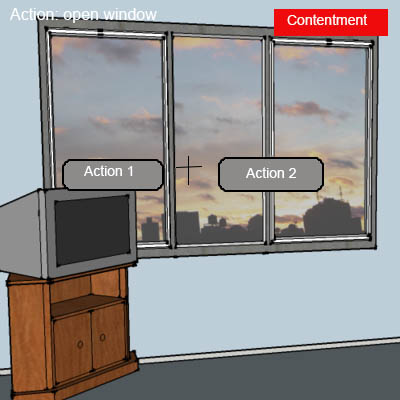
\includegraphics[scale=0.5]{images/design/interface_actions.jpg}
\caption{Mock up of contentment and action selection}
\label{design_interface_actions}
\end{figure}

Controls will be standard game controls commonly found in games. This should minimise learning involved in playing the game,  for current and novice game player alike: 

\begin{enumerate}
\item Mouse or direction buttons will be used to control the camera
\item W: move forward
\item S: move backwards
\item A: move left
\item D: move right
\item Space bar: action button for interacting with objects
\end{enumerate}

\subsection{User tasks: Mission and Explore mode}
Two modes in the simulator will be created, "Explore mode" and "Mission mode". Explore mode offers the user an opportunity to navigate the environment whilst learning how to deal hazards such as sensory overloads and meltdowns with less penalty than in the Mission mode. Explanations, hints and suggestions will be offered as the user has difficulty, for example after the first meltdown an explanation will occur explaining what has happened and that this occurs when contentment reaches zero. On the second meltdown occurrence a hint will be offered as a means to potentially avoid these in the future. In addition, this highlights interview-obtained information that children with high-functioning autism were unable to pinpoint what was causing them to meltdown until they were older and able to verbalise; they had to learn how to avoid situation through experience. 

Mission mode is a game mode that requires the user to complete specific tasks, apply and test their acquired knowledge and understanding from the explore mode whilst circumventing obstacles, in essence, this is the game or story mode of the program. Meta-cognition can be defined as "Knowledge about knowledge" and holds two key elements: Knowledge about knowledge, knowledge regulation which entails formulating plans as to fill knowledge gaps. By implementing the two different game-modes, an environment to learn and then later test it should aid meta-cognitive knowledge development in respect to autism. Users could acquire their own skills and strategies in dealing with these situations, and if some of their conclusions to dealing with these strategies are similar to someone with autism, it will aid understanding as to why some of the autism coping strategies are used.  

For the prototype version of the game, the Mission mode will entail two tasks: To get dressed and then proceed to obtaining a drink from the kitchen and hazards in the kitchen will include lights and a washing machine which will be placed next to the sink. For the first complete version a more in depth storyboard will be created with the aid of feedback from people whom have autism. 

\section{Simulator features}

\subsection{Description boxes}
Users will be able to click on certain objects and obtain information in the form of pop up boxes that may be of interest, hazardous or cause problems for someone with autism. I.e explaining that information on TV may be taken literally and a child may thus expect a toy to react in the same way as advertised or may not be able to identify that what is seen on TV is not real or explaining that clothes can literally feel like sandpaper. This information will be taken from literature and suggestions from people with Autism. 

\subsection{Sensory overloads}
Three sensory-types will be implemented; sound, light and tactile. The proximity and amount of objects around the player will firstly affect the sensory health(which is not visible to the user). When this falls below a specified threshold the first level of a sensory overload occurs and the impact of surrounding objects become more prominent, lights becoming brighter even if they were not initially interfering and causing the sensory overload and the contentment will slowly start to reduce. If the player does not move away, the second level is reached and the contentment bar reduction is rapid; visual effects worsen as the environment becomes more troublesome to navigate; representing a full sensory overload.

Following mock-ups and the positive response, two versions of a sensory overload were implemented and recorded before being sent via email to adults with autism to acquire feedback. The first was not well received or understood, however the second which was much closer to the previous mock images in \ref{sensorymockup3} had a strong positive response.  

One of the effects of sensory overloads was for lights to get brighter which can be easily conveyed in JMonkey using "Bloom" filters. A Guassian filter is suggested to make the overall environment harder to navigate and to mirror dizziness described when experiencing a full sensory overload. 

Finally, the sensory system will effect and be affected by the contentment bar. Interviews showed that if someone with autism is feeling particularly drained from their day or awakens feeling particularly anxious their tolerance to surroundings is lower and hence when contentment is lower, a sensory overload is more likely to occur. If the user is around no interferences or people, contentment will slowly increase. 

\subsection{Meltdowns}
Meltdowns occur when someone with Autism becomes stressed or overwhelmed. This will be represented as 'Contentment' drawing comparison to a "health bar", commonly seen in games. There have been multiple suggestions to convey this:

\begin{itemize}
\item During a meltdown, make the character harder to control. When pushing "right" the character instead moves left and vice versa.
\item Make the screen blackout and reopen with items in the house destroyed.
\end{itemize}

The first option was selected and moulded for the prototype. As contentment gets closer to zero, the camera will shake, giving the player a few seconds to attempt to prevent the meltdown. The closer contentment gets to zero the more the camera will shake. When contentment reaches zero, a meltdown will occur and the player will restart in the bedroom. 

\subsection{Special interests}
'Special interests' were chosen as a way to alleviate some of the difficulties within the environment and replenish contentment. When engaging with a special interest, troublesome sounds will be reduced and if experiencing a sensory overload or meltdown the effects will subsidise. The special interest selected will be a Dinosaur toy which the user can interact with.

\subsection{Information processing delay}
Information processing delay was highlighted in interviews by a teacher as one of the main causes of meltdowns in school. When the user clicks on an object to interact or is expected to give a response, actions will be made harder to select by rotation around the screen. If the character has lower contentment the selections will move even quicker which should result in a greater delay from the player as it becomes more difficult to click them. Such delays could later affect responses from other characters in the game; if the user does not respond quick enough an in-game character such as the parent will prompt the user to hurry up, causing contentment to further drop and the actions to rotate quicker. It was highlighted in the lit review that if someone with autism is interrupted during information processing, they have to start over again but it becomes harder due to stress and anxiety. 

\section{Tool selection}
A game engine was selected to allow focus to be directed onto higher level concepts of the simulator. Suitable game engine candidates as well as modelling tools were identified by looking at those highly rated on gamedev.net (extensive online resource for game developers), whilst taking some previous knowledge into account. After narrowing choices to a few, the advantages and disadvantages were weight up and a choice was finally made. 

\subsection{Game engines}

\begin{table}[H]
    \begin{tabular}{| p{2cm} | p{4cm} | p{6cm} | p{5cm}| }
    \hline
    Engine & Description & Advantages & Disadvantages \\ \hline
    Unity & Unity is one of the most popular game engines available with good support for models. Unfortunately the licence costs 1500 and the free version comes with limitations. & \begin{minipage}{6cm}
    \vskip 4pt
    \begin{enumerate}
   \item Popular game engine to use with a large support base and model repository. 
   \item Quick development with scripting, games with impressive graphics can be made quickly. 
   \item Phone app support.
   \end{enumerate}
   \vskip 4pt
 \end{minipage}   & 
 \begin{minipage}{5cm}
    \vskip 4pt
    \begin{enumerate}
   \item Interface heavy 
   \item Limited to scripting rather than having control of whole game architecture
   \item Costs 
   \item Good computer required to run it efficiently.
   \end{enumerate}
   \vskip 4pt
 \end{minipage}
	\\ \hline
	JMonkey & JMonkey is a java 3d game engine that has been in development around for a few years. It has an extremely active and helpful community, allows complete customisation and holds little limitation being open source.  &
	 \begin{minipage}{6cm}
    \vskip 4pt
    \begin{enumerate}
   \item Provides development environment in addition to a scene graph.
   \item Active community where you often get responses from developers themselves.
   \item Java is quick to develop in enabling focus on higher level features.
   \item Support for online use and phone apps aiding goals of accessibility.  
   \end{enumerate}
   \vskip 4pt
 \end{minipage}  
 & 
 	 \begin{minipage}{5cm}
    \vskip 4pt
    \begin{enumerate}
   \item Java is not seen as the preferred language for graphics or games.
   \end{enumerate}
   \vskip 4pt
 \end{minipage}  \\ \hline
 Panda3D & Originally created by Disney, Panda3D is an engine which can be used via python or C++ although support is mostly for python. & 	 \begin{minipage}{6cm}
    \vskip 4pt
    \begin{enumerate}
   \item Quick to develop for with a choice in language.
   \item Good community with lots of tools.
   \end{enumerate}
   \vskip 4pt
 \end{minipage} &  \begin{minipage}{5cm}
    \vskip 4pt
    \begin{enumerate}
   \item No phone app and limited online support. 
   \item Lack of documentation. 
   \end{enumerate}
   \vskip 4pt
 \end{minipage}
    \\ \hline
    Ogre3D & Ogre3d is primarily a graphics rendering engine and but it does have additional plugins such as 'physics' or drawing interfaces &  \begin{minipage}{6cm}
    \vskip 4pt
    \begin{enumerate}
   \item Lots of modules and plugins
   \item Active support community
   \item Open-source
   \end{enumerate}
   \vskip 4pt
 \end{minipage}
 &  \begin{minipage}{5cm}
    \vskip 4pt
    \begin{enumerate}
   \item Longer development process
   \item Lack of tools such as a scene graph. 
   \item No online support
   \end{enumerate}
   \vskip 4pt
 \end{minipage}
    \end{tabular}
\end{table}

JMonkey was chosen for its active community, development environment being open source and programmed in Java and open-source. Although Java is not seen as the programming language of choice for graphics it enables quicker development than C++ counterparts. Unity allows speedy quick development with great results but the pro version would be required for some features which is very expensive. As JMonkey is in Java put online with ease, increasing accessibility. Finally there were no foreseen limitations with using JMonkey a part from concerns about performance which may become an issue at a later date.

\subsection{Modelling tools}
For modelling there several options available:
\begin{itemize}
\item Maya
\item 3DSMax
\item Blender
\item Sketchup
\end{itemize}

Both Maya and 3DSMax are considered the industries leaders in modelling, animations and effect creation. However, they are both extremely expensive, costing over £3000. Sketchup is a google product, giving a wealth of models however its ease of use for beginners comes at a cost; it is not well supported for games although sketch-up models can be ported to other modelling software and edited to be more suited. Blender is an open source 3D modelling program with quick updates and the choice of tool for many game developers although has been thought to have a steeper learning curve than 3DSMax.

Blender was selected as the primary modelling tool for the creation of game assets, as there is little lost in using it in-spite of being free. It is widely used by game developers and professionals and is the tool JMonkey is most built to accommodate.